\documentclass[aspectratio=169,11pt]{beamer}

\usepackage[utf8]{inputenc}
\usepackage[T1]{fontenc}
\usepackage[spanish,es-noshorthands,es-nodecimaldot]{babel}
\usepackage{lmodern}
\usepackage[scaled=0.92]{helvet}
\usepackage{amsmath,amssymb,bm}
\usepackage{graphicx}
\usepackage{tikz}
\usetikzlibrary{calc,positioning,arrows.meta,shapes.geometric}
\usepackage{pgfplots}
\pgfplotsset{compat=1.18}

\renewcommand{\ttdefault}{lmtt}
\hyphenpenalty=10000
\exhyphenpenalty=10000

\definecolor{classicblue}{HTML}{0F4C81}
\definecolor{vivamagenta}{HTML}{BB2649}
\definecolor{clouddance}{HTML}{F0EEE9}
\definecolor{tinta}{HTML}{1B2733}
\definecolor{grismedio}{HTML}{5E6873}
\colorlet{azulnoche}{classicblue!62!black}

\newcommand{\figs}{../report/figures}
\newcommand{\demourl}{https://unet-tumor-segmentation-jruano-adelgado.streamlit.app/}
\newcommand{\fs}[2]{\fontsize{#1}{#2}\selectfont}
\newcommand{\pct}{\,\symbol{37}}
\newcommand{\vlambda}{\bm{\lambda}}
\newcommand{\vtheta}{\bm{\theta}}
\newcommand{\ra}{$\bm{\rightarrow}$}
\DeclareMathOperator*{\argmax}{arg\,m\acute{a}x}
\DeclareMathOperator*{\argmin}{arg\,m\acute{\imath}n}

\setbeamertemplate{navigation symbols}{}
\setbeamersize{text margin left=8mm,text margin right=8mm}
\setbeamercolor{normal text}{fg=tinta,bg=white}
\setbeamercolor{frametitle}{fg=classicblue}
\setbeamercolor{framesubtitle}{fg=grismedio}
\setbeamerfont{frametitle}{size=\fs{17}{20},series=\bfseries}
\setbeamerfont{framesubtitle}{size=\fs{7.5}{9},series=\bfseries}
\setbeamertemplate{frametitle}{\vspace{4.8mm}\hbox to\textwidth{\raisebox{-1.1mm}{\color{vivamagenta}\rule{1.4mm}{5.6mm}}\hspace{2.8mm}{\usebeamerfont{frametitle}\usebeamercolor[fg]{frametitle}\insertframetitle}\hfill{\usebeamerfont{framesubtitle}\insertframesubtitle}}\vspace{0.6mm}}
\setbeamertemplate{footline}{\hbox to\paperwidth{\hspace{8mm}{\fs{6.5}{8}\color{grismedio}Optimización en dos niveles para la segmentación de tumores cerebrales en RM}\hfill{\fs{6.5}{8}\color{grismedio}\insertframenumber\,/\,\inserttotalframenumber}\hspace{8mm}}\vspace{3.4mm}}

\tikzset{
  lienzo/.style={x=1mm,y=1mm,line cap=round,line join=round},
  txt/.style={inner sep=0pt,outer sep=0pt,align=flush left,text=tinta},
  flecha/.style={-{Stealth[length=2.2mm,width=1.8mm]},line width=0.8pt,draw=classicblue},
  paso/.style={draw=classicblue,line width=0.7pt,fill=white,minimum width=38mm,minimum height=9mm,align=center,inner sep=1pt,font=\fs{8}{9.6},text=classicblue},
  foto/.style={inner sep=0pt,outer sep=0pt},
}

\newcommand{\kpicard}[7]{
  \fill[clouddance] (#1,#2) rectangle ++(#3,#4);
  \fill[#5] (#1,#2) rectangle ++(1.2,#4);
  \node[txt,anchor=north west,font=\fs{17}{19}\bfseries,text=#5] at ($(#1,#2)+(4,#4-3.4)$) {#6};
  \node[txt,anchor=north west,font=\fs{7}{8.6},text=grismedio,text width=#3mm-6mm] at ($(#1,#2)+(4,#4-11.6)$) {#7};
}

\newcommand{\tarjeta}[5]{
  \fill[clouddance] (#1,#2) rectangle ++(#3,#4);
  \fill[#5] (#1,#2) rectangle ++(1.2,#4);
}

\title{Optimización en dos niveles para la segmentación de tumores cerebrales en RM}
\author{Javier Ruano Hernández, Alejandro Delgado Valera}
\institute{Universidad de Las Palmas de Gran Canaria}
\subject{Optimización y Heurística}

\newcommand{\interno}{{\color{classicblue}NIVEL INTERNO}}
\newcommand{\externo}{{\color{vivamagenta}NIVEL EXTERNO}}

\begin{document}

\begin{frame}[plain]
\begin{tikzpicture}[remember picture,overlay,lienzo,shift={(current page.south west)}]
  \node[foto,anchor=south west] at (100,60) {\includegraphics[width=30mm,height=30mm,trim=14bp 184bp 296.4bp 13.9bp,clip]{\figs/mri_examples.pdf}};
  \node[foto,anchor=south west] at (130,60) {\includegraphics[width=30mm,height=30mm,trim=14bp 32bp 296.4bp 165.9bp,clip]{\figs/mri_examples.pdf}};
  \node[foto,anchor=south west] at (100,30) {\includegraphics[width=30mm,height=30mm,trim=161.5bp 184bp 149.4bp 13.9bp,clip]{\figs/mri_examples.pdf}};
  \node[foto,anchor=south west] at (130,30) {\includegraphics[width=30mm,height=30mm,trim=161.5bp 32bp 149.4bp 165.9bp,clip]{\figs/mri_examples.pdf}};
  \node[foto,anchor=south west] at (100,0) {\includegraphics[width=30mm,height=30mm,trim=308.5bp 184bp 1.9bp 13.9bp,clip]{\figs/mri_examples.pdf}};
  \node[foto,anchor=south west] at (130,0) {\includegraphics[width=30mm,height=30mm,trim=308.5bp 32bp 1.9bp 165.9bp,clip]{\figs/mri_examples.pdf}};
  \draw[white,line width=0.5mm,line cap=butt] (130,0) -- (130,90);
  \draw[white,line width=0.5mm,line cap=butt] (100,30) -- (160,30);
  \draw[white,line width=0.5mm,line cap=butt] (100,60) -- (160,60);
  \draw[white,line width=0.5mm,line cap=butt] (100,0) -- (100,90);
  \foreach \y/\t in {61.6/Meningioma,31.6/Glioma,1.6/Hipofisario} {
    \node[anchor=south west,inner xsep=1.4mm,inner ysep=0.9mm,fill=black,fill opacity=0.6,text opacity=1,text=white,font=\fs{6.5}{8}\bfseries] at (101.6,\y) {\t};
  }
  \node[txt,anchor=north west,font=\fs{8}{10}\bfseries,text=vivamagenta] (kicker) at (10,77) {OPTIMIZACIÓN Y HEURÍSTICA};
  \node[txt,anchor=north west,font=\fs{20}{24.5}\bfseries,text=classicblue,text width=84mm] (titulo) at (10,70.5) {Optimización en dos niveles para la segmentación de tumores cerebrales en RM};
  \fill[vivamagenta] ($(titulo.south west)+(0,-4.4)$) rectangle ++(18,1.1);
  \node[txt,anchor=north west,font=\fs{10.5}{14}\bfseries] (autores) at ($(titulo.south west)+(0,-9)$) {Javier Ruano Hernández\\Alejandro Delgado Valera};
  \node[txt,anchor=south west,font=\fs{8}{10},text=grismedio] at (10,7.5) {Universidad de Las Palmas de Gran Canaria};
\end{tikzpicture}
\end{frame}

\begin{frame}{El problema y los datos}{CONTEXTO}
\centering
\begin{tikzpicture}[lienzo]
  \useasboundingbox (0,0) rectangle (143,64);
  \node[foto,anchor=south west] at (0,5.7) {\includegraphics[width=70mm]{\figs/mri_examples.pdf}};
  \node[foto,anchor=north west] at (74,58.3) {\includegraphics[width=69mm]{\figs/dataset_split.pdf}};
  \kpicard{74}{5.7}{21.6}{22}{classicblue}{3064}{cortes T1-CE \textperiodcentered{} 233 pacientes}
  \kpicard{97.7}{5.7}{21.6}{22}{vivamagenta}{1.7\pct}{píxeles tumorales}
  \tarjeta{121.4}{5.7}{21.6}{22}{classicblue}
  \fill[classicblue] (125.4,18.4) rectangle ++(9.6,5.2);
  \fill[vivamagenta] (135.4,18.4) rectangle ++(2.4,5.2);
  \fill[white] (138.2,18.4) rectangle ++(2.9,5.2);
  \draw[classicblue,line width=0.5pt] (138.2,18.4) rectangle ++(2.9,5.2);
  \node[txt,anchor=north west,font=\fs{7}{8.6},text=grismedio,text width=15.6mm] at (125.4,16.1) {Partición estricta por paciente};
\end{tikzpicture}
\end{frame}

\begin{frame}{Enfoque: optimización en dos niveles}{ENFOQUE}
\centering
\begin{tikzpicture}[lienzo]
  \useasboundingbox (0,0) rectangle (143,64);
  \tarjeta{0}{42}{143}{22}{vivamagenta}
  \tarjeta{0}{0}{143}{22}{classicblue}
  \node[txt,anchor=west,font=\fs{7.5}{9}\bfseries,text=vivamagenta] at (6,58.2) {NIVEL EXTERNO};
  \node[txt,anchor=west,font=\fs{12}{14}\bfseries,text=classicblue] at (6,52.6) {Algoritmo genético};
  \node[txt,anchor=west,font=\fs{8}{10},text=grismedio] at (6,47.2) {búsqueda de hiperparámetros};
  \node[txt,anchor=center,font=\fs{13}{16}] at (80,53) {$\displaystyle \vlambda^{\star}\in\argmax_{\vlambda}\;\mathsf{Dice}_{\mathsf{val}}\bigl(\vtheta^{\star}(\vlambda)\bigr)$};
  \node[txt,anchor=east,font=\fs{17}{19}\bfseries,text=vivamagenta] at (138,55.4) {4};
  \node[txt,anchor=east,font=\fs{7}{8.6},text=grismedio] at (138,48.6) {variables, sin gradiente};
  \node[txt,anchor=west,font=\fs{7.5}{9}\bfseries,text=classicblue] at (6,16.2) {NIVEL INTERNO};
  \node[txt,anchor=west,font=\fs{12}{14}\bfseries,text=classicblue] at (6,10.6) {U-Net + Adam};
  \node[txt,anchor=west,font=\fs{8}{10},text=grismedio] at (6,5.2) {descenso por gradiente};
  \node[txt,anchor=center,font=\fs{13}{16}] at (80,11) {$\displaystyle \vtheta^{\star}(\vlambda)\in\argmin_{\vtheta}\;\mathcal{L}_{\mathsf{ent}}(\vtheta;\vlambda)$};
  \node[txt,anchor=east,font=\fs{17}{19}\bfseries,text=classicblue] at (138,13.4) {10\textsuperscript{6}--10\textsuperscript{7}};
  \node[txt,anchor=east,font=\fs{7}{8.6},text=grismedio] at (138,6.6) {pesos, gradiente exacto};
  \draw[flecha,draw=vivamagenta,line width=1.3pt] (56,41) -- (56,23);
  \draw[flecha,line width=1.3pt] (104,23) -- (104,41);
  \node[txt,anchor=east,align=right,font=\fs{10}{12}] at (53,33.6) {$\vlambda=(\eta,\lambda,F,D)$};
  \node[txt,anchor=east,align=right,font=\fs{7}{8.6},text=grismedio] at (53,28.8) {hiperparámetros};
  \node[txt,anchor=west,font=\fs{10}{12}] at (107,33.6) {$\mathsf{Dice}_{\mathsf{val}}$};
  \node[txt,anchor=west,font=\fs{7}{8.6},text=grismedio] at (107,28.8) {aptitud};
  \node[txt,anchor=center,font=\fs{9}{11}\itshape,text=grismedio] at (80,32) {sujeto a};
\end{tikzpicture}
\end{frame}

\begin{frame}{Arquitectura U-Net}{\interno}
\centering
\begin{tikzpicture}[
    lienzo,
    enc/.style={fill=classicblue,draw=classicblue,line width=0.5pt,inner sep=0pt},
    dec/.style={fill=classicblue!16,draw=classicblue,line width=0.7pt,inner sep=0pt},
    can/.style={txt,font=\fs{7.5}{9},text=grismedio},
    salto/.style={-{Stealth[length=2.2mm,width=1.8mm]},line width=1.1pt,draw=vivamagenta,dash pattern=on 2.2pt off 1.6pt},
  ]
  \useasboundingbox (0,0) rectangle (143,64);
  \node[enc,minimum width=3.2mm,minimum height=12mm] (e0) at (30,56) {};
  \node[enc,minimum width=4.6mm,minimum height=10mm] (e1) at (40,42) {};
  \node[enc,minimum width=6.4mm,minimum height=8mm] (e2) at (50,30) {};
  \node[enc,minimum width=8.6mm,minimum height=6.6mm] (e3) at (60,19.7) {};
  \node[enc,minimum width=12mm,minimum height=5.4mm] (b) at (72.5,10.7) {};
  \node[dec,minimum width=8.6mm,minimum height=6.6mm] (d3) at (85,19.7) {};
  \node[dec,minimum width=6.4mm,minimum height=8mm] (d2) at (95,30) {};
  \node[dec,minimum width=4.6mm,minimum height=10mm] (d1) at (105,42) {};
  \node[dec,minimum width=3.2mm,minimum height=12mm] (d0) at (115,56) {};
  \node[dec,fill=white,minimum width=2mm,minimum height=12mm] (c) at (122.5,56) {};
  \node[foto] (x) at (10,56) {\includegraphics[width=13mm,height=13mm,trim=2bp 20.5bp 342.1bp 14.3bp,clip]{\figs/segmentation_comparison.pdf}};
  \node[foto] (p) at (136,56) {\includegraphics[width=13mm,height=13mm,trim=342bp 20.5bp 2.1bp 14.3bp,clip]{\figs/segmentation_comparison.pdf}};
  \node[can,anchor=north] at (10,48.4) {RM \textperiodcentered{} $256^{2}$};
  \node[can,anchor=north] at (136,48.4) {4 clases};
  \node[can,anchor=east] at ($(e0.west)+(-1.2,-3.6)$) {$F$};
  \node[can,anchor=east] at ($(e1.west)+(-1.2,0)$) {$2F$};
  \node[can,anchor=east] at ($(e2.west)+(-1.2,0)$) {$4F$};
  \node[can,anchor=east] at ($(e3.west)+(-1.2,0)$) {$8F$};
  \node[can,anchor=north] at ($(b.south)+(0,-1.4)$) {$16F$};
  \node[can,anchor=west] at ($(d3.east)+(1.2,0)$) {$8F$};
  \node[can,anchor=west] at ($(d2.east)+(1.2,0)$) {$4F$};
  \node[can,anchor=west] at ($(d1.east)+(1.2,0)$) {$2F$};
  \node[can,anchor=west] at ($(d0.east)+(0.6,-8.2)$) {$F$};
  \draw[flecha] (x.east) -- (e0.west);
  \draw[flecha] (d0.east) -- (c.west);
  \draw[flecha] (c.east) -- (p.west);
  \draw[flecha] (e0.south) -- (e1.north);
  \draw[flecha] (e1.south) -- (e2.north);
  \draw[flecha] (e2.south) -- (e3.north);
  \draw[flecha] (e3.south) -- (b.north west);
  \draw[flecha] (b.north east) -- (d3.south);
  \draw[flecha] (d3.north) -- (d2.south);
  \draw[flecha] (d2.north) -- (d1.south);
  \draw[flecha] (d1.north) -- (d0.south);
  \draw[salto] (e0.east) -- (d0.west);
  \draw[salto] (e1.east) -- (d1.west);
  \draw[salto] (e2.east) -- (d2.west);
  \draw[salto] (e3.east) -- (d3.west);
  \node[txt,anchor=center,font=\fs{9}{11}\bfseries,text=vivamagenta] at (72.5,49.2) {conexiones de salto};
  \node[enc,minimum width=2.6mm,minimum height=3.4mm] at (2.3,17.2) {};
  \node[can,anchor=west] at (6.4,17.2) {codificador};
  \node[dec,minimum width=2.6mm,minimum height=3.4mm] at (2.3,11.2) {};
  \node[can,anchor=west] at (6.4,11.2) {decodificador};
  \draw[flecha] (2.3,7) -- (2.3,3);
  \node[can,anchor=west] at (6.4,5) {\emph{pooling} / interpolación};
  \kpicard{100}{0}{43}{21}{vivamagenta}{1.8\,M -- 7.2\,M}{parámetros ($F=16 \rightarrow F=32$)}
\end{tikzpicture}
\end{frame}

\begin{frame}{Objetivo y descenso}{\interno}
\centering
\begin{tikzpicture}[lienzo]
  \useasboundingbox (0,0) rectangle (143,64);
  \foreach \x in {0,49,98} {
    \tarjeta{\x}{0}{45}{64}{classicblue}
  }
  \node[txt,anchor=west,font=\fs{10.5}{12.5}\bfseries,text=classicblue] at (5,58) {Pérdida Focal Tversky};
  \node[txt,anchor=west,font=\fs{10.5}{12.5}\bfseries,text=classicblue] at (54,58) {Optimizador Adam};
  \node[txt,anchor=west,font=\fs{10.5}{12.5}\bfseries,text=classicblue] at (103,58) {\emph{Cosine annealing}};

  \fill[grismedio] (20.4,29) -- (25.6,29) -- (23,34.6) -- cycle;
  \draw[tinta,line width=1.3pt] (8,31.7) -- (38,37.5);
  \fill[vivamagenta] (12,38.4) circle (5.6);
  \fill[classicblue] (34,40.9) circle (4);
  \node[txt,anchor=center,font=\fs{8.5}{10}\bfseries,text=white] at (12,38.4) {FN};
  \node[txt,anchor=center,font=\fs{7.5}{9}\bfseries,text=white] at (34,40.9) {FP};
  \node[txt,anchor=center,font=\fs{8.5}{10}\bfseries,text=vivamagenta] at (11,25.6) {$\alpha=0.6$};
  \node[txt,anchor=center,font=\fs{8.5}{10}\bfseries,text=classicblue] at (35,25.6) {$\beta=0.4$};
  \node[txt,anchor=center,font=\fs{8.5}{10}] at (23,15.2) {$\mathsf{TI}=\dfrac{\mathsf{TP}}{\mathsf{TP}+\alpha\,\mathsf{FN}+\beta\,\mathsf{FP}}$};
  \node[txt,anchor=west,font=\fs{7.5}{9},text=grismedio] at (5,4.6) {Omitir tumor penaliza más};

  \begin{scope}
    \clip (51,23) rectangle (93,53);
    \foreach \a/\b/\o in {21/10.5/14,16/8/22,11/5.5/32,6.4/3.2/46,2.4/1.2/70} {
      \draw[classicblue!\o,line width=0.8pt,rotate around={18:(80,33)}] (80,33) ellipse [x radius=\a,y radius=\b];
    }
    \draw[vivamagenta,line width=1.2pt,-{Stealth[length=2mm,width=1.7mm]}] plot[smooth,tension=0.6] coordinates {(55,49) (60,42.4) (65,41.6) (69,37.6) (74,36.2) (79.2,33.3)};
    \foreach \p in {(55,49),(60,42.4),(65,41.6),(69,37.6),(74,36.2)} {
      \fill[vivamagenta] \p circle (0.75);
    }
  \end{scope}
  \node[txt,anchor=center,font=\fs{8.5}{10}] at (72,15.2) {$\vtheta_{t}=\vtheta_{t-1}-\eta\,\dfrac{\hat{\mathbf{m}}_{t}}{\sqrt{\hat{\mathbf{v}}_{t}}+\epsilon}$};
  \node[txt,anchor=west,font=\fs{7.5}{9},text=grismedio] at (54,4.6) {Inercia y paso adaptativo};

  \draw[grismedio,line width=0.6pt,-{Stealth[length=1.8mm,width=1.5mm]}] (106,26) -- (140,26);
  \draw[grismedio,line width=0.6pt,-{Stealth[length=1.8mm,width=1.5mm]}] (106,26) -- (106,53);
  \draw[grismedio!70,line width=0.7pt,dash pattern=on 1.6pt off 1.4pt] (106,49) -- (137,49);
  \draw[vivamagenta,line width=1.5pt] plot[domain=0:1,samples=50] ({106+31*\x},{26+11.5*(1+cos(180*\x))});
  \node[txt,anchor=east,font=\fs{7.5}{9},text=grismedio] at (105,49) {$\eta_{0}$};
  \node[txt,anchor=north,font=\fs{7}{8.6},text=grismedio] at (137,24.8) {$T$};
  \node[txt,anchor=north,font=\fs{7}{8.6},text=grismedio] at (121.5,24.8) {época};
  \node[txt,anchor=south east,font=\fs{6.5}{8},text=grismedio] at (137,49.8) {constante};
  \node[txt,anchor=center,font=\fs{8.5}{10}] at (120.5,15.2) {$\eta_{e}=\dfrac{\eta_{0}}{2}\Bigl(1+\cos\dfrac{\pi e}{T}\Bigr)$};
  \node[txt,anchor=west,font=\fs{7.5}{9},text=grismedio] at (103,4.6) {Oscilación del Dice: $0.022 \rightarrow 0.003$};
\end{tikzpicture}
\end{frame}

\begin{frame}{Cromosoma del AG}{\externo}
\centering
\begin{tikzpicture}[
    lienzo,
    fila/.style={txt,anchor=west,font=\fs{8.5}{10}\bfseries,text=classicblue},
    sub/.style={txt,anchor=west,font=\fs{7.5}{9},text=grismedio},
    mini/.style={txt,anchor=center,font=\fs{7.5}{9},text=grismedio},
    valor/.style={txt,anchor=center,font=\fs{10.5}{12.5}\bfseries,text=vivamagenta},
  ]
  \useasboundingbox (0,0) rectangle (143,64);
  \node[anchor=east,rounded corners=2.8mm,fill=clouddance,inner xsep=3.6mm,inner ysep=0pt,minimum height=5.6mm,font=\fs{7.5}{9},text=grismedio] at (143,61) {\textbf{\color{classicblue}46} evaluaciones \textperiodcentered{} \textbf{\color{classicblue}3} épocas / evaluación};

  \node[fila] at (0,50) {Genotipo};
  \node[sub] at (0,45.2) {$\mathbf{u}\in[0,1]^{4}$};
  \node[fila] at (0,33.4) {Decodificación};
  \node[sub] at (0,28.6) {$\vlambda=\varphi(\mathbf{u})$};
  \node[fila] at (0,14.8) {Fenotipo};
  \node[sub] at (0,10) {mejor solución};

  \fill[classicblue] (27,41.5) rectangle (143,54);
  \foreach \x in {56,85,114} {
    \draw[white,line width=0.9pt,line cap=butt] (\x,41.5) -- (\x,54);
  }
  \foreach \i/\v/\n in {1/0.249/tasa de aprendizaje,2/0.094/decaimiento de pesos,3/0.478/filtros base,4/0.520/profundidad} {
    \pgfmathsetmacro{\cx}{27+29*(\i-1)+14.5}
    \node[txt,anchor=center,font=\fs{7.5}{9},text=white] at (\cx,50.8) {$u_{\i}$};
    \node[txt,anchor=center,font=\fs{12}{14}\bfseries,text=white] at (\cx,45.6) {\v};
    \draw[flecha] (\cx,40.4) -- (\cx,36.8);
    \draw[flecha] (\cx,24.6) -- (\cx,21);
    \fill[clouddance] (\cx-13.6,5) rectangle (\cx+13.6,19.8);
    \fill[vivamagenta] (\cx-13.6,5) rectangle (\cx+13.6,5.9);
    \node[mini] at (\cx,9.6) {\n};
  }

  \foreach \cx/\u/\lo/\hi in {41.5/0.249/-4/-2,70.5/0.094/-6/-3} {
    \draw[grismedio,line width=0.9pt] (\cx-9.5,31.6) -- (\cx+9.5,31.6);
    \draw[grismedio,line width=0.9pt] (\cx-9.5,30.2) -- (\cx-9.5,33);
    \draw[grismedio,line width=0.9pt] (\cx+9.5,30.2) -- (\cx+9.5,33);
    \fill[vivamagenta] (\cx-9.5+19*\u,31.6) circle (1.5);
    \node[mini] at (\cx-9.5,27.2) {$10^{\lo}$};
    \node[mini] at (\cx+9.5,27.2) {$10^{\hi}$};
  }
  \foreach \cx/\ta/\tb/\tc in {99.5/8/16/32,128.5/3/4/5} {
    \draw[grismedio,line width=0.6pt] (\cx-10.5,27.4) rectangle ++(7,7);
    \draw[grismedio,line width=0.6pt] (\cx+3.5,27.4) rectangle ++(7,7);
    \fill[vivamagenta] (\cx-3.5,27.4) rectangle ++(7,7);
    \node[txt,anchor=center,font=\fs{8.5}{10},text=grismedio] at (\cx-7,30.9) {\ta};
    \node[txt,anchor=center,font=\fs{8.5}{10}\bfseries,text=white] at (\cx,30.9) {\tb};
    \node[txt,anchor=center,font=\fs{8.5}{10},text=grismedio] at (\cx+7,30.9) {\tc};
  }

  \node[valor] at (41.5,14.6) {$\eta=3.15\cdot10^{-4}$};
  \node[valor] at (70.5,14.6) {$\lambda=1.91\cdot10^{-6}$};
  \node[valor] at (99.5,14.6) {$F=16$};
  \node[valor] at (128.5,14.6) {$D=4$};
\end{tikzpicture}
\end{frame}

\begin{frame}{Flujo evolutivo y operadores}{\externo}
\centering
\begin{tikzpicture}[
    lienzo,
    nombre/.style={txt,anchor=center,align=flush center,font=\fs{7.5}{9}\bfseries,text=classicblue,text width=18.5mm},
    param/.style={txt,anchor=center,font=\fs{8.5}{10}\bfseries,text=vivamagenta},
    nota/.style={txt,font=\fs{7}{8.6},text=grismedio},
  ]
  \useasboundingbox (0,0) rectangle (143,64);
  \node[paso] (ini) at (19,59.3) {\textbf{Población inicial}\\[-0.3mm]{\fs{6.5}{8}\color{grismedio}$N=10$, con siembra}};
  \node[paso] (eva) at (19,46.6) {\textbf{Evaluación}\\[-0.3mm]{\fs{6.5}{8}\color{grismedio}aptitud: 3 épocas}};
  \node[paso,shape=diamond,aspect=2.4,minimum width=31mm,minimum height=13mm,inner sep=0pt] (dec) at (19,27) {\textbf{¿$g=5$?}};
  \node[paso,fill=vivamagenta,draw=vivamagenta,text=white] (fin) at (19,5) {\textbf{Mejor} $\vlambda^{\star}$};
  \draw[flecha] (ini) -- (eva);
  \draw[flecha] (eva) -- (dec);
  \draw[flecha] (dec) -- (fin);
  \node[nota,anchor=west] at (20.6,14.6) {sí};
  \node[nota,anchor=south] at (39.6,27.8) {no};

  \foreach \x in {45,70.5,96,121.5} {
    \tarjeta{\x}{11}{21.5}{32}{classicblue}
  }
  \draw[flecha] (dec.east) -- (44.4,27);
  \foreach \x in {67.1,92.6,118.1} {
    \draw[flecha] (\x,27) -- ++(2.8,0);
  }
  \draw[flecha] (132.25,43.6) -- (132.25,46.6) -- (eva.east);
  \node[nota,anchor=south] at (86,47.6) {nueva población, $g \leftarrow g+1$};

  \node[nombre] at (56.3,21.6) {Torneo};
  \node[param] at (56.3,15.4) {$k=3$};
  \node[nombre] at (81.8,21.6) {Cruce BLX-$\alpha$};
  \node[param] at (81.8,15.4) {$\alpha=0.5$};
  \node[nombre] at (107.3,21.6) {Mutación gaussiana};
  \node[param] at (107.3,15.4) {$\sigma=0.2$};
  \node[nombre] at (132.8,21.6) {Elitismo};
  \node[param] at (132.8,15.4) {$e=1$};

  \fill[classicblue!40] (49.8,28.6) rectangle ++(3.2,5);
  \fill[vivamagenta] (54.7,28.6) rectangle ++(3.2,10.4);
  \fill[classicblue!40] (59.6,28.6) rectangle ++(3.2,7);
  \draw[grismedio,line width=0.6pt] (48.6,28.6) -- (64,28.6);

  \fill[vivamagenta!22] (73.8,31.4) rectangle (89.8,35.4);
  \fill[classicblue!38] (77.8,31.4) rectangle (85.8,35.4);
  \fill[classicblue] (77.8,33.4) circle (1.25);
  \fill[classicblue] (85.8,33.4) circle (1.25);
  \fill[vivamagenta] (88,33.4) circle (1.25);
  \draw[grismedio,line width=0.6pt] (73.8,29.6) -- (89.8,29.6);

  \draw[classicblue,line width=1pt] plot[domain=-8:8,samples=40] ({107.3+\x},{29+10*exp(-\x*\x/9)});
  \draw[grismedio,line width=0.6pt] (99.3,29) -- (115.3,29);
  \fill[classicblue] (107.3,29) circle (1.25);
  \fill[vivamagenta] (111.6,29) circle (1.25);

  \fill[vivamagenta] (127.4,38) circle (1.5);
  \fill[classicblue!40] (127.4,33.6) circle (1.5);
  \fill[classicblue!40] (127.4,29.2) circle (1.5);
  \fill[vivamagenta] (138.2,38) circle (1.5);
  \draw[classicblue,line width=0.7pt] (138.2,33.6) circle (1.3);
  \draw[classicblue,line width=0.7pt] (138.2,29.2) circle (1.3);
  \draw[flecha,draw=vivamagenta] (129.8,38) -- (135.9,38);
\end{tikzpicture}
\end{frame}

\begin{frame}{Resultados del AG y diagnóstico}{\externo}
\centering
\begin{tikzpicture}[lienzo]
  \useasboundingbox (0,0) rectangle (143,64);
  \begin{axis}[
      at={(11mm,29.5mm)},
      anchor=south west,
      scale only axis,
      width=66mm,
      height=32mm,
      xmin=0.7,xmax=5.3,
      ymin=0.2,ymax=0.56,
      xtick={1,2,3,4,5},
      ytick={0.2,0.3,0.4,0.5},
      xlabel={Generación},
      ylabel={Aptitud},
      axis lines=left,
      axis line style={draw=grismedio!70,line width=0.5pt,-},
      tick style={draw=grismedio!70},
      tick label style={font=\fs{7}{8.6},text=grismedio},
      label style={font=\fs{7.5}{9},text=grismedio},
      ymajorgrids,
      grid style={draw=clouddance,line width=0.7pt},
      clip=false,
    ]
    \addplot[classicblue,line width=1.1pt,mark=*,mark size=1.4pt] coordinates {(1,0.2464) (2,0.2983) (3,0.3327) (4,0.3560) (5,0.3370)};
    \addplot[vivamagenta,line width=1.7pt,mark=*,mark size=1.9pt] coordinates {(1,0.4409) (2,0.4409) (3,0.5085) (4,0.5085) (5,0.5085)};
    \node[anchor=west,inner sep=0pt,font=\fs{7.5}{9}\bfseries,text=vivamagenta] at (axis cs:5.16,0.5085) {mejor};
    \node[anchor=west,inner sep=0pt,font=\fs{7.5}{9}\bfseries,text=classicblue] at (axis cs:5.16,0.337) {media};
    \node[anchor=south,inner sep=1.4pt,font=\fs{7.5}{9}\bfseries,text=vivamagenta] at (axis cs:1,0.452) {0.441};
    \node[anchor=south,inner sep=1.4pt,font=\fs{7.5}{9}\bfseries,text=vivamagenta] at (axis cs:3,0.52) {0.509};
  \end{axis}
  \kpicard{0}{0}{46}{19.5}{vivamagenta}{0.441\,\ra\,0.509}{mejor aptitud en 46 evaluaciones}
  \kpicard{48.5}{0}{38.5}{19.5}{classicblue}{3.2$\bm{\times}$}{convergencia más rápida}

  \fill[clouddance] (92,0) rectangle (143,64);
  \fill[vivamagenta] (92,0) rectangle (93.6,64);
  \node[txt,anchor=west,font=\fs{10.5}{12.5}\bfseries,text=vivamagenta] at (97.5,57.6) {Sesgo de horizonte corto};
  \node[txt,anchor=west,font=\fs{8.5}{10}\bfseries,text=classicblue] at (97.5,46.6) {$F=16$};
  \fill[vivamagenta] (110,44.2) rectangle ++(20.36,4.8);
  \node[txt,anchor=west,font=\fs{8.5}{10}\bfseries,text=vivamagenta] at (131.4,46.6) {0.509};
  \node[txt,anchor=west,font=\fs{8.5}{10}\bfseries,text=classicblue] at (97.5,38.6) {$F=32$};
  \fill[classicblue] (110,36.2) rectangle ++(17.62,4.8);
  \node[txt,anchor=west,font=\fs{8.5}{10}\bfseries,text=classicblue] at (128.7,38.6) {0.441};
  \draw[grismedio,line width=0.6pt] (110,34.6) -- (110,50.6);
  \node[txt,anchor=west,font=\fs{7}{8.6},text=grismedio] at (97.5,30) {aptitud a 3 épocas, mismo $(\eta,\lambda)$};
  \draw[grismedio!45,line width=0.5pt] (97.5,24.6) -- (138.5,24.6);
  \foreach \y/\t in {18.4/Premia la velocidad inicial,11.6/Penaliza redes grandes,4.8/No ve el \emph{cosine annealing}} {
    \fill[vivamagenta] (97.5,\y-0.9) rectangle ++(1.8,1.8);
    \node[txt,anchor=west,font=\fs{8}{10}] at (101.6,\y) {\t};
  }
\end{tikzpicture}
\end{frame}

\begin{frame}{Refinamiento guiado}{FASES 5 Y 6}
\centering
\begin{tikzpicture}[
    lienzo,
    idx/.style={txt,anchor=center,font=\fs{19}{21}\bfseries,text=classicblue!30},
    tit/.style={txt,anchor=west,font=\fs{9}{11}\bfseries,text=classicblue},
    val/.style={txt,anchor=west,font=\fs{9.5}{11.5}\bfseries,text=vivamagenta},
    sub/.style={txt,anchor=west,font=\fs{6.8}{8.4},text=grismedio},
  ]
  \useasboundingbox (0,0) rectangle (143,64);
  \foreach \x/\y in {0/43,44.5/43,0/20,44.5/20} {
    \tarjeta{\x}{\y}{42}{21}{classicblue}
  }
  \node[idx] at (7,53.5) {1};
  \node[tit] at (12.4,59) {Aumento espacial};
  \node[val] at (12.4,52.8) {12.2\pct\,\ra\,8.0\pct};
  \node[sub] at (12.4,47.4) {gliomas omitidos};
  \node[idx] at (51.5,53.5) {2};
  \node[tit] at (56.9,59) {Capacidad $F{=}32$};
  \node[val] at (56.9,52.8) {1.8\,M\,\ra\,7.2\,M};
  \node[sub] at (56.9,47.4) {parámetros};
  \node[idx] at (7,30.5) {3};
  \node[tit] at (12.4,36) {\emph{Cosine annealing}};
  \node[val] at (12.4,29.8) {0.022\,\ra\,0.003};
  \node[sub] at (12.4,24.4) {oscilación del Dice};
  \node[idx] at (51.5,30.5) {4};
  \node[tit] at (56.9,36) {Pesos $\alpha{=}0.6$, $\beta{=}0.4$};
  \node[val] at (56.9,29.8) {2.25\,\ra\,1.11};
  \node[sub] at (56.9,24.4) {FN/FP en glioma};

  \node[txt,anchor=west,font=\fs{7}{8.6},text=grismedio] at (0,13.4) {AG (A)};
  \node[txt,anchor=west,font=\fs{17}{19}\bfseries,text=classicblue] at (0,6) {0.776};
  \draw[flecha,line width=1.3pt] (22,6) -- (61,6);
  \node[txt,anchor=south,font=\fs{7.5}{9}\bfseries,text=classicblue] at (41.5,7.6) {Dice en prueba};
  \node[txt,anchor=east,font=\fs{7}{8.6},text=grismedio] at (86.5,13.4) {Refinado (E)};
  \node[txt,anchor=east,font=\fs{17}{19}\bfseries,text=vivamagenta] at (86.5,6) {0.818};

  \node[foto,anchor=south east] at (143,4.4) {\includegraphics[width=52mm]{\figs/conf_matrix_E.pdf}};
\end{tikzpicture}
\end{frame}

\begin{frame}{Resultados finales y segmentación visual}{RESULTADOS}
\centering
\begin{tikzpicture}[lienzo]
  \useasboundingbox (0,0) rectangle (143,63.5);
  \node[foto,anchor=north] at (71.5,63.5) {\includegraphics[width=124mm]{\figs/segmentation_comparison.pdf}};
  \node[txt,anchor=west,font=\fs{6.8}{8.4},text=grismedio] at (0,20.4) {DICE MEDIO EN PRUEBA};
  \foreach \v in {0.70,0.75,0.80,0.85} {
    \pgfmathsetmacro{\gx}{32+(\v-0.65)*180}
    \draw[clouddance,line width=0.7pt] (\gx,0.4) -- (\gx,18.2);
  }
  \foreach \y/\n/\v/\c/\s in {15.9/Manual/0.691/grismedio/\mdseries,11.3/AG (A)/0.776/classicblue/\mdseries,6.7/Refinado (E)/0.818/vivamagenta/\bfseries,2.1/ResNet34 (F)/0.825/classicblue/\mdseries} {
    \pgfmathsetmacro{\px}{32+(\v-0.65)*180}
    \node[txt,anchor=west,font=\fs{8}{10}\s,text=tinta] at (0,\y) {\n};
    \draw[\c!35,line width=1.2pt] (32,\y) -- (\px,\y);
    \fill[\c] (\px,\y) circle (1.35);
    \node[txt,anchor=west,font=\fs{8.5}{10}\bfseries,text=\c] at (72,\y) {\v};
  }
  \kpicard{88}{0}{26.5}{20.4}{vivamagenta}{$\bm{\approx}$\,64\pct}{de la mejora total, por el AG}
  \kpicard{116.5}{0}{26.5}{20.4}{classicblue}{0.8175}{Dice, entrenado desde cero}
\end{tikzpicture}
\end{frame}

\begin{frame}{Conclusiones y trabajo futuro}{CIERRE}
\centering
\begin{tikzpicture}[
    lienzo,
    num/.style={txt,anchor=west,font=\fs{24}{26}\bfseries},
    tit/.style={txt,anchor=west,font=\fs{10}{12}\bfseries,text=classicblue},
    sub/.style={txt,anchor=north west,font=\fs{8}{10.4},text=grismedio,text width=37mm},
    futuro/.style={rounded corners=3.4mm,fill=white,draw=classicblue,line width=0.8pt,minimum height=6.8mm,inner xsep=4mm,inner ysep=0pt,font=\fs{8.5}{10}\bfseries,text=classicblue},
  ]
  \useasboundingbox (0,0) rectangle (143,64);
  \tarjeta{0}{25}{45}{39}{vivamagenta}
  \tarjeta{49}{25}{45}{39}{classicblue}
  \tarjeta{98}{25}{45}{39}{classicblue}
  \node[num,text=vivamagenta] at (5,54.6) {64\pct};
  \node[tit] at (5,43.2) {Sinergia de dos niveles};
  \node[sub] at (5,38.2) {AG explora; el gradiente ajusta};
  \node[num,text=classicblue] at (54,54.6) {0.8175};
  \node[tit] at (54,43.2) {Auditar la heurística};
  \node[sub] at (54,38.2) {Corregir el sesgo: $+0.041$ Dice};
  \node[num,text=classicblue] at (103,54.6) {7$\bm{\times}$};
  \node[tit] at (103,43.2) {\emph{Transfer learning}};
  \node[sub] at (103,38.2) {Complemento: converge antes, Dice empatado};

  \node[txt,anchor=west,font=\fs{7.5}{9}\bfseries,text=vivamagenta] at (0,16.6) {TRABAJO FUTURO};
  \draw[flecha,line width=1.1pt] (0,7) -- (143,7);
  \node[futuro] at (24,7) {Multi-fidelidad};
  \node[futuro] at (71.5,7) {Cromosoma ampliado};
  \node[futuro] at (117,7) {NSGA-II};
\end{tikzpicture}
\end{frame}

{
\setbeamercolor{background canvas}{bg=classicblue}
\begin{frame}[plain]
\begin{tikzpicture}[remember picture,overlay,lienzo,shift={(current page.south west)}]
  \foreach \y/\x in {60/130,30/100,0/70} {
    \begin{scope}
      \clip (130,\y) rectangle ++(30,30);
      \node[foto,anchor=south west] at (\x,\y) {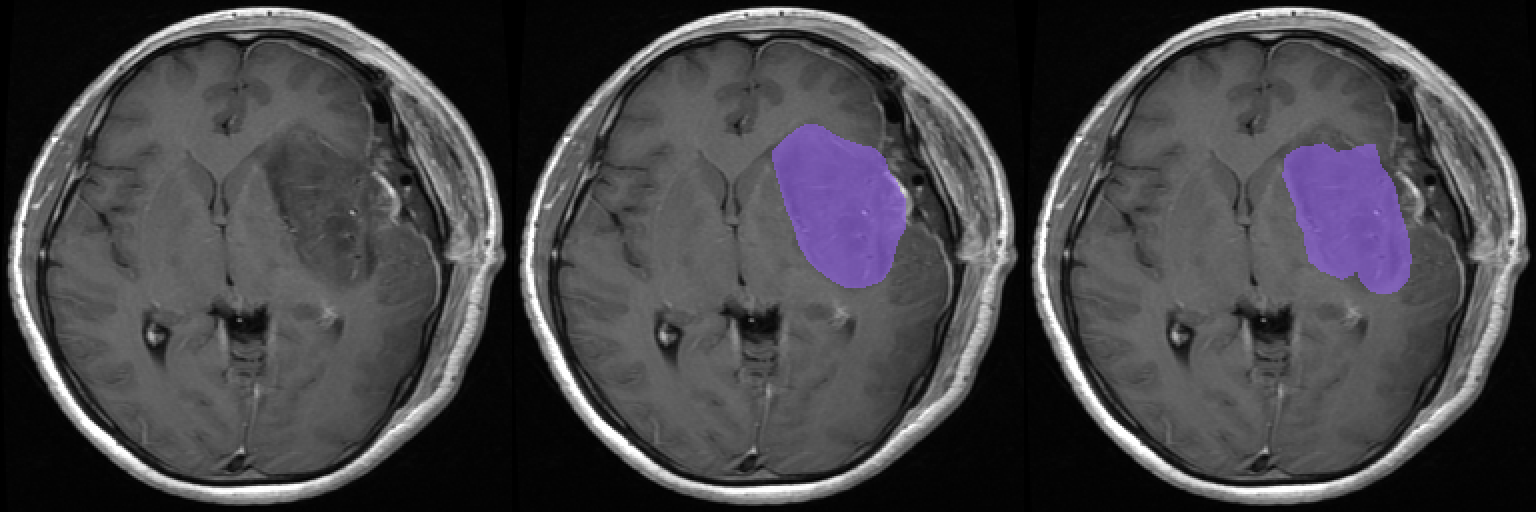
\includegraphics[width=90mm,height=30mm]{../hero_overlay.png}};
    \end{scope}
  }
  \draw[classicblue,line width=0.5mm,line cap=butt] (130,0) -- (130,90);
  \draw[classicblue,line width=0.5mm,line cap=butt] (130,30) -- (160,30);
  \draw[classicblue,line width=0.5mm,line cap=butt] (130,60) -- (160,60);

  \node[txt,anchor=north west,font=\fs{8}{10}\bfseries,text=white] at (10,79) {STREAMLIT};
  \node[txt,anchor=north west,font=\fs{27}{31}\bfseries,text=white] (titulo) at (10,73) {Demostración en vivo};
  \fill[vivamagenta] (10,58.8) rectangle ++(18,1.1);

  \fill[azulnoche,rounded corners=1.6mm] (10,39) rectangle (120,54.5);
  \node[txt,anchor=west,font=\fs{15}{18}\ttfamily\bfseries,text=vivamagenta!55!white] at (15.5,46.75) {\$};
  \node[txt,anchor=west,font=\fs{15}{18}\ttfamily\bfseries,text=white] at (22.5,46.75) {streamlit run app/main.py};
  \node[foto,anchor=south west] at (10,39) {\href{\demourl}{\makebox[110mm]{\rule{0pt}{15.5mm}}}};
  \fill[vivamagenta!55!white] (11.4,34.6) circle (0.9);
  \node[txt,anchor=west,font=\fs{8}{10}\ttfamily,text=white] at (14.2,34.6) {\href{\demourl}{\color{white}unet-tumor-segmentation-jruano-adelgado.streamlit.app}};

  \foreach \x/\n/\t in {10/1/Segmentación\\en tiempo real,47.5/2/Comparativa\\Base vs. E vs. F,85/3/Superposición de máscaras} {
    \draw[white,line width=0.6pt,opacity=0.55] (\x,8) rectangle ++(35,17);
    \fill[vivamagenta] (\x+5.6,16.5) circle (3.1);
    \node[txt,anchor=center,font=\fs{9}{11}\bfseries,text=white] at (\x+5.6,16.5) {\n};
    \node[txt,anchor=west,font=\fs{8.5}{10.6}\bfseries,text=white,text width=23mm] at (\x+10.6,16.5) {\t};
  }
\end{tikzpicture}
\end{frame}
}

\end{document}
